\documentclass[10pt,twocolumn]{article}

% use the oxycomps style file
\usepackage{oxycomps}

% other packages
\usepackage{algorithm}
\usepackage{algorithmic}

% read references.bib for the bibtex data
\bibliography{references}

% include metadata in the generated pdf file
\pdfinfo{
    /Title (Tutorial Report)
    /Author (Adrian Manhey)
}

% set the title and author information
\title{Tutorial Report: Reinforcement Learning Using OpenAI's Gym Environment}
\author{Adrian Manhey}
\affiliation{Occidental College}
\email{amanhey.edu}

\begin{document}

\maketitle

% Introduction

This tutorial \cite{tutorial} report follows an article from LearnDataSci, written by Satwik Kansal and Brendan Martin, a Software Developer and founder of LearnDataSci, respectively.
The goal of the tutorial was to solve OpenAI Gym's Taxi problem, which OpenAI describes as "there are 4 locations (labeled by different letters), and our job is to pick up the passenger at one location and drop him off at another. We receive +20 points for a successful drop-off and lose 1 point for every time-step it takes. There is also a 10 point penalty for illegal pick-up and drop-off actions." \cite{Taxi-v3}

% Methods

\section{Methods}

In Figure \ref{Figure 1} we can see a sample state of the taxi game.
The colored square represents the taxi, which is yellow without a passenger and green with a passenger.
The pipe represents a wall which the taxi cannot cross.
The letters R, G, Y, B are the possible pickup and destination locations, where the blue letter represents the current passenger pick-up location, and the purple letter is the current destination.

\begin{figure}[ht]
    \caption{State 328 of Taxi Game}
    \centering
    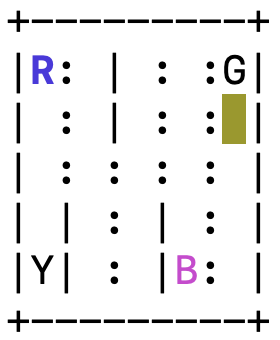
\includegraphics[width=0.15\textwidth]{frame.png}
    \label{Figure 1}
\end{figure}

This frame is a rendering of the observable space of the game, i.e. what can be rendered to humans, and corresponds to the $328^{\text{th}}$ state of this game.
When designing the environment one of the first things to consider is where the observable space is going to be discrete, e.g. grid based environments like this taxi game, or continuous, where the position of the agent is represented by real-valued coordinates.
The action space can also be discrete or continuous, the distinct taxi actions are discrete since there is no action between going up and right in this game, while in the mobile app game Angry Birds \cite{AngryBirds} the amount of force applied on the slingshot is continuous.
For the taxi game, the action space is 6 due to the 4 directions we are able to move and the pick-up and the drop-off actions.
We have 500 state spaces due to the 5x5 grid with 25 possible taxi locations, 5 passenger locations (including inside the taxi), and 4 pick-up/drop-off locations.

Initially, the Gym environment creates a reward table for all the possible action and state combinations, which it labels as $P$.
The initial reward table at state 328 can be seen in Table \ref{Table:1}.
The reward table comes in the form, \[ \{\text{action: [ probability, nextstate, reward, done ]} \} \]
The actions are encoded from 0 to 5 for the directions (South, North, East, West) and pick-up and drop-off.
One thing to notice is that if the taxi tries to go with action 2 (moving west) the next state would be the current state (328) but a negative penalty would be incurred.
Since this is the initial table all the probabilities (weights) of each action are the same.

The first method the tutorial examined to complete this task was a "brute force" method which involved picking random actions until the goal was reached.
This method was able to solve the task but had a relatively large number of epochs and penalties.
To improve this the tutorial introduced reinforcement learning for the task.

\subsection{Q-learning}
% Reinforcement Learning
This reinforcement learning program was implemented with a Q-learning algorithm that looks at an action taken from a particular state and updates a value, called a \textbf{Q-value} in a table to see if that action was beneficial.
All the Q-values are stored in a Q-table that are associated with a state and action pair $(s, a)$, representing the "quality" of an action at a state.
Q-values are initialized to an arbitrary value, 1 in this tutorial, and as the agent explores the environment they are updated.
The method for updating a Q-value consists of two parameters: $\alpha \in (0, 1]$ is the learning rate and $\gamma \in [0, 1]$ is the discount factor, which makes short-term or long-term rewards more valuable.
The equation for this relationship can be written as \[ Q(s, a) = (1 - \alpha)Q(s, a) + \alpha(r + \gamma \text{max}Q_a(s', A)),\] where $r$ is the reward of an action, $s'$ is the next state, and $A$ is all the possible actions that can be taken.
So we are learning the proper action by taking the old Q-value and adding the learned value of the immediate reward and possible future rewards.

\begin{algorithm}
\label{Algorithm: 1}
\caption{Q-Learning Algorithm}
\begin{algorithmic}
\REQUIRE $Q, \alpha, \gamma, \epsilon$
\FOR{$i \in N$}
\STATE $\text{random } s \leftarrow S$
\WHILE{end state not reached}
\IF{$ \text{random number } < \epsilon$}
\STATE $\text{random } a \leftarrow A$
\ELSE
\STATE $a = \text{max}_a(Q[s])$
\ENDIF
\STATE $s', r = \text{step}(a)$
\STATE $Q_i = Q[s, a]$
\STATE $Q[s, a] = (1 - \alpha) * Q_i + \alpha * (r + \gamma *  \text{max}Q[s'])$
\STATE $s = s'$
\ENDWHILE
\RETURN $Q$
\ENDFOR
\end{algorithmic}
\end{algorithm}

The implementation, seen in Algorithm \ref{Algorithm: 1}, has our Q-table defined as $Q$ and uses two loops, one to iterate through the number of episodes $N$ and one for epochs.
The difference between the two is that the number of episodes is the amount of scenarios the algorithm is learning from, whereas the epochs are the steps in an episode.
The tutorial trained on 100,000 episodes where each episode started with the taxi being generated at a random position on the grid.
Notably, in the implementation there is an additional parameter $\epsilon$, which can be thought of the exploration parameter.
This tells the algorithm how often to pick a random action instead of the current most beneficial one from the Q-table.

%P-table
\begin{table}[ht]
    \vspace{1cm}
    \centering
    \caption{Looking at P-values}
    \label{Table:1}
    \begin{tabular}{ || c c c c c|| }
      \hline
        Action & P-value & Next State & Penalty & Done \\ \hline \hline
        0 & 1.0 & 428 & -1 & False \\ \hline
        1 & 1.0 & 228 & -1 & False \\ \hline
        2 & 1.0 & 348 & -1 & False \\ \hline
        3 & 1.0 & 328 & -1 & False \\ \hline
        4 & 1.0 & 328 & -10 & False \\ \hline
        5 & 1.0 & 328 & -10 & False \\ \hline
    \end{tabular}
\end{table}

%Q-table
\begin{table}[ht]
    \vspace{1cm}
    \centering
    \caption{Looking at Q-values for State 328}
    \label{Table:2}
    \begin{tabular}{ || c c || }
      \hline
        Action & Q-value \\ \hline \hline
        0 & -2.412 \\ \hline
        1 & -2.273 \\ \hline
        2 & -2.411 \\ \hline
        3 & -2.362 \\ \hline
        4 & -9.560 \\ \hline
        5 & -10.43 \\ \hline
    \end{tabular}
\end{table}


After training all of the Q-values for the states visited during an episode are updated and we can see in Table \ref{Table:2} that at our 328 state the best action our agent has learned to do is action 2 (North), which from Figure \ref{Figure 1} is a reasonable move.

\section{Evaluation Metrics}

The main evaluation metrics for this game were the time needed to complete the game (epochs) and reward received, which is impacted by the number of penalties.
Although the tutorial mentions evaluation the ratio of reward to time, the metrics in this section were not part of the original tutorial.

% Brute Force Evaluation
Over 1000 iterations of the brute force method, the average number of epochs required to complete the task was $742.689$ while the average number of penalties was $239.697$.
It is notable that this method was able to complete the game but the range of epochs and penalties was quite wide, where epochs ranged from 2 to 14572 and penalties 0 to 4701.
For the games on the lower end, the passenger and taxi were created in the same spot and the random action correctly chose pick-up and then drop-off.
For the games on the high end, the taxi moved around the grid but failed to use the pick-up and drop-off actions at the correct points so it would "circle" the grid.

% Reinforcement Learning Evaluation

Evaluating the performance of the RL algorithm, \ref{Table:3} has the averages of the number of epochs required for the $10^i$th, $i \in [0, 1, 2, 3, 4],$ episode and the number of penalties incurred.
When the algorithm begins it performs similarly to the brute force method, however as the episodes increase the number of epochs and penalties steadily decreases.

\begin{table}[ht]
    \vspace{1cm}
    \centering
    \caption{Averages from 50 Iterations of RL}
    \label{Table:3}
    \begin{tabular}{ || c c c || }
       \hline
       Episode & Epochs & Penalties  \\ \hline \hline
       1 & 608.44 & 93.08  \\ \hline
       10 & 874.22 & 55.36 \\ \hline
       100 & 224.14 & 7.7 \\ \hline
       1000 & 29.1 & 0.78 \\ \hline
       10000 & 13.56 & 0.42 \\ \hline
    \end{tabular}
\end{table}

\section{Results and Discussion}

After training we can see that in 100 episodes, the average number epochs and penalties have drastically decreased from 4147 to 13.29 and 1372 to 0, respectively.
This decrease shows that our model does much better than the brute force algorithm and is able to avoid mistakes it has made before.
At the end, our result is the generated Q-table which holds all the Q-values for our state and action pairs.
This can be referenced in order to successfully, as seen, complete the task with the goal of optimizing the amount of time taken and reward received.

In order to optimize our parameters we can modify them in a couple ways: (1) decrease the learning rate as the knowledge base increases, (2) decrease the discount factor as we get closer to the end since the long-term reward becomes a short-term reward, and (3) decrease the exploration parameter as the number of trials increase. We can do this by selecting parameters beforehand using something similar to GridSearch to optimize reward/time steps because we want the greatest reward as fast as possible. We might also want to optimize for the number of penalties incurred.

After completing this tutorial I have a better understanding of how to implement a Q-learning algorithm in Python and next steps will to be to create a custom environment in Gym for my project.
Additionally I have steps I have methods to compare, such as the brute force method, and know steps I can take to optimize the parameters.

\printbibliography

\end{document}
